%----------------------------------------------------------------------------------------
%	PACKAGES AND OTHER DOCUMENT CONFIGURATIONS
%----------------------------------------------------------------------------------------

\documentclass[12pt]{article}

\usepackage{polski}
\usepackage[polish]{babel}
\usepackage[utf8]{inputenc}
\usepackage{datetime}
\usepackage{graphicx} 
\usepackage{tikz}
\usepackage{amsmath} 
\usepackage{epstopdf}
\usepackage{multirow} 
\usepackage{tabularx}
%\usepackage[colorlinks=true]{hyperref}
%\usepackage[all]{hypcap}
%\usepackage{showframe} 
\usepackage{geometry}
 \geometry{
 	a4paper, 
 	left	=20mm,
 	right	=20mm,
 	top		=20mm,
 	bottom	=20mm,
 }
 
%----------------------------------------------------------------------------------------
 
%----------------------------------------------------------------------------------------
% DATES
%----------------------------------------------------------------------------------------

\renewcommand{\dateseparator}{.}
\newdate{exercise_date}{20}{10}{2014}

%----------------------------------------------------------------------------------------

%----------------------------------------------------------------------------------------
% TIKZ PACKAGES
%----------------------------------------------------------------------------------------

\usetikzlibrary{arrows}

%----------------------------------------------------------------------------------------

\begin{document}
 
\begin{titlepage}

\newcommand{\HRule}{\rule{\linewidth}{0.5mm}}
% Defines a new command for the horizontal lines, change thickness here

\center
% Center everything on the page
 
%----------------------------------------------------------------------------------------
%	LOGO SECTION
%----------------------------------------------------------------------------------------

\includegraphics[width=6cm]{../res/img/logo.png}\\[1cm]
% Include a department/university logo - this will require the graphicx package
 
%----------------------------------------------------------------------------------------
 
%----------------------------------------------------------------------------------------
%	HEADING SECTIONS
%----------------------------------------------------------------------------------------

\textsc{\LARGE Akademia Górniczo-Hutnicza \\[0.2cm]
im. Stanisława Staszica w Krakowie}\\[1.5cm]
% Name of your university/college

\textrm{\Large Wydział Elektrotechniki Automatyki Informatyki i Inżynierii
Biomedycznej}\\[1cm]

\textsc{\Large Laboratorium Aparatury Automatyzacji}\\[0.5cm]
% Major heading such as course name

%----------------------------------------------------------------------------------------
%	TITLE SECTION
%----------------------------------------------------------------------------------------

\HRule \\[0.4cm]
{ \huge \bfseries Prosty regulator mikroprocesorowy 
}\\%[0.4cm]
% Title of your document
\HRule \\[1.5cm]

%----------------------------------------------------------------------------------------
%	REPORT TABLE
%----------------------------------------------------------------------------------------

\begin{table}[h]
\centering
\begin{tabularx}{\linewidth}{|c|l|X|}
\hline
% \multicolumn{3}{|c|}{
% \begin{tabular}{cc}
% \begin{tabular}{c}
% \includegraphics[height=2.2cm]{../res/img/logo.jpg}\\
% \end{tabular}
% &
% \begin{tabular}{c}
% \Large{Akademia Górniczo-Hutnicza im. Stanisława Staszica}\\[5pt]
% \large{\textsc{Katedra Automatyki}}\\[5pt]
% \textsc{Laboratorium Aparatury Automatyzacji}
% \end{tabular}
% \end{tabular}
% }\\
% \hline
% \multicolumn{3}{|c|}{}\\[-5pt]
% \multicolumn{3}{|c|}{\textbf{\huge{Ćwiczenie 6}}}\\[10pt]
% \multicolumn{3}{|c|}{\Large{Bezpośrednie sterowanie cyfrowe}}\\[8pt]
% \hline
\multicolumn{2}{|c|}{Wydział EAIiIB, kierunek AiR, rok II}
& Grupa 6, wtorek 11:00-12:30\\
\hline
Lp. & Imię i nazwisko & Zaliczenie\\
\hline
1 & \textbf{Konrad Adasiewicz} & \\
\hline
2 & \textbf{Michał Maciejewski} & \\
\hline
3 & \textbf{Bartosz Szmit} & \\
\hline
\multicolumn{2}{|c|}{Data wykonania ćwiczenia:
\ddmmyyyydate\displaydate{exercise_date}r.} & Data oddania sprawozdania:
\ddmmyyyydate\displaydate{create_date}r.
\\
\hline
\end{tabularx}
\end{table}

%----------------------------------------------------------------------------------------

\vfill % Fill the rest of the page with whitespace

\end{titlepage} 

% Program ćwiczenia

\begin{section}{Program ćwiczenia}
	\begin{enumerate}
	  	\item Konfiguracja i badanie przemysłowego pirometrycznego
					   przetwornika temperatury
		\begin{itemize}
			\item Wyznaczenie współczynnika emisyjności obiektu pomiaru
			\item Określenie wpływu współczynnika emisyjności na wynik pomiaru
			\item Wpływ przesłon ograniczających bezpośrednie oddziaływanie
			promieniowania temperaturowego na pirometr
		\end{itemize}
		\item Rejestracja mierzonej temperatury i wyznaczenie odpowiedzi
			  dynamicznej pirometru
		\item Nastawianie oraz odczyt parametrów pirometru z
			  wykorzystaniem interfejsu portu szeregowego
	\end{enumerate}
\end{section}

\begin{section}{Przebieg ćwiczenia}
	\begin{subsection}{Wyznaczenie współczynnika emisyjności obiektu pomiaru}
		Celem wyznaczenia współczynnika emisyjności został wykonany pomiar temperatury
		obiektu wzorcowego o znanej emisyjności, oznaczmy tę temperaturę $T_0$.
		Następnie wykonany został pomiar temperatury obiektu, którego emisyjność badaliśmy, o
		którym wiedzieliśmy, iż posiada taką samą temperaturę jak obiekt wzorcowy.
		Pomiar ten był obarczony błędem związanym z nieprawidłowym współczynnikiem
		emisyjności wprowadzonym w oprogramowanie przeliczające odczyty pirometru na
		rzeczywistą temperaturę. Pomiar był wykonywany dopóki nie został dobrany taki
		współczynnik emisyjności, aby odczyt temperatury badanego obiektu był równy
		$T_0$. Dobrany współczynnik emisyjności jest współczynnikiem badanego obiektu.
		
		W przypadku przeprowadzanego ćwiczenia obiekt wzorcowy i obiekt badany były
		tożsame, mianowicie były to kubki z gorącą wodą z miejscowo zakrytą
		powierzchnią materiałem o znanej emisyjności.
		
		Podczas ćwiczenia wyznaczyliśmy współczynniki emisyjności trzech badanych
		obiektów. Zostały uzyskane następujące wyniki:
		\begin{itemize}
		  \item Kubek żółty $\varepsilon = 0.69[-]$
		  \item Kubek zielony $\varepsilon = 0.87[-]$
		  \item Kubek niebieski $\varepsilon = 0.82[-]$
		\end{itemize}
	\end{subsection}
	
	\newpage
	
	\begin{subsection}{Określenie wpływu współczynnika emisyjności na wynik
	pomiaru}
		Zostały wykonane pomiary temperatury obiektu o stałej emisyjności, przy czym
		każdy pomiar został wykonany dla innego przyjętego do obliczeń wykonywanych
		wewnątrz przetwornika pomiarowego współczynnika emisyjności. Zatem nie została
		sprawdzona rzeczywista fizyczna zależność temperatury od współczynnika
		emisyjności obiektu, lecz wprowadzona przez producenta pirometru
		zależność wykorzystana do przeliczenia odczytów wewnętrznych na rzeczywistą
		temperaturę.
		
		Zmierzona temperatura obiektu zależy od współczynnika emisyjności badanego
		obiektu. W instrukcji podana jest zależność, którą można przedstawić w
		uproszczonej formie:
		\begin{equation}
			T = \sqrt[4]{\dfrac{C}{\varepsilon}}
			\label{equ:temp}
		\end{equation}
		gdzie $C$ jest pewną stałą. Jak widać dla $\varepsilon \approx 0$ pomiar
		temperatury może być obarczony znacznym błędem wynikającym z niedokładności
		pomiaru samego współczynnika emisyjności obiektu.
		\begin{figure}[!htb]
			\begin{center}
				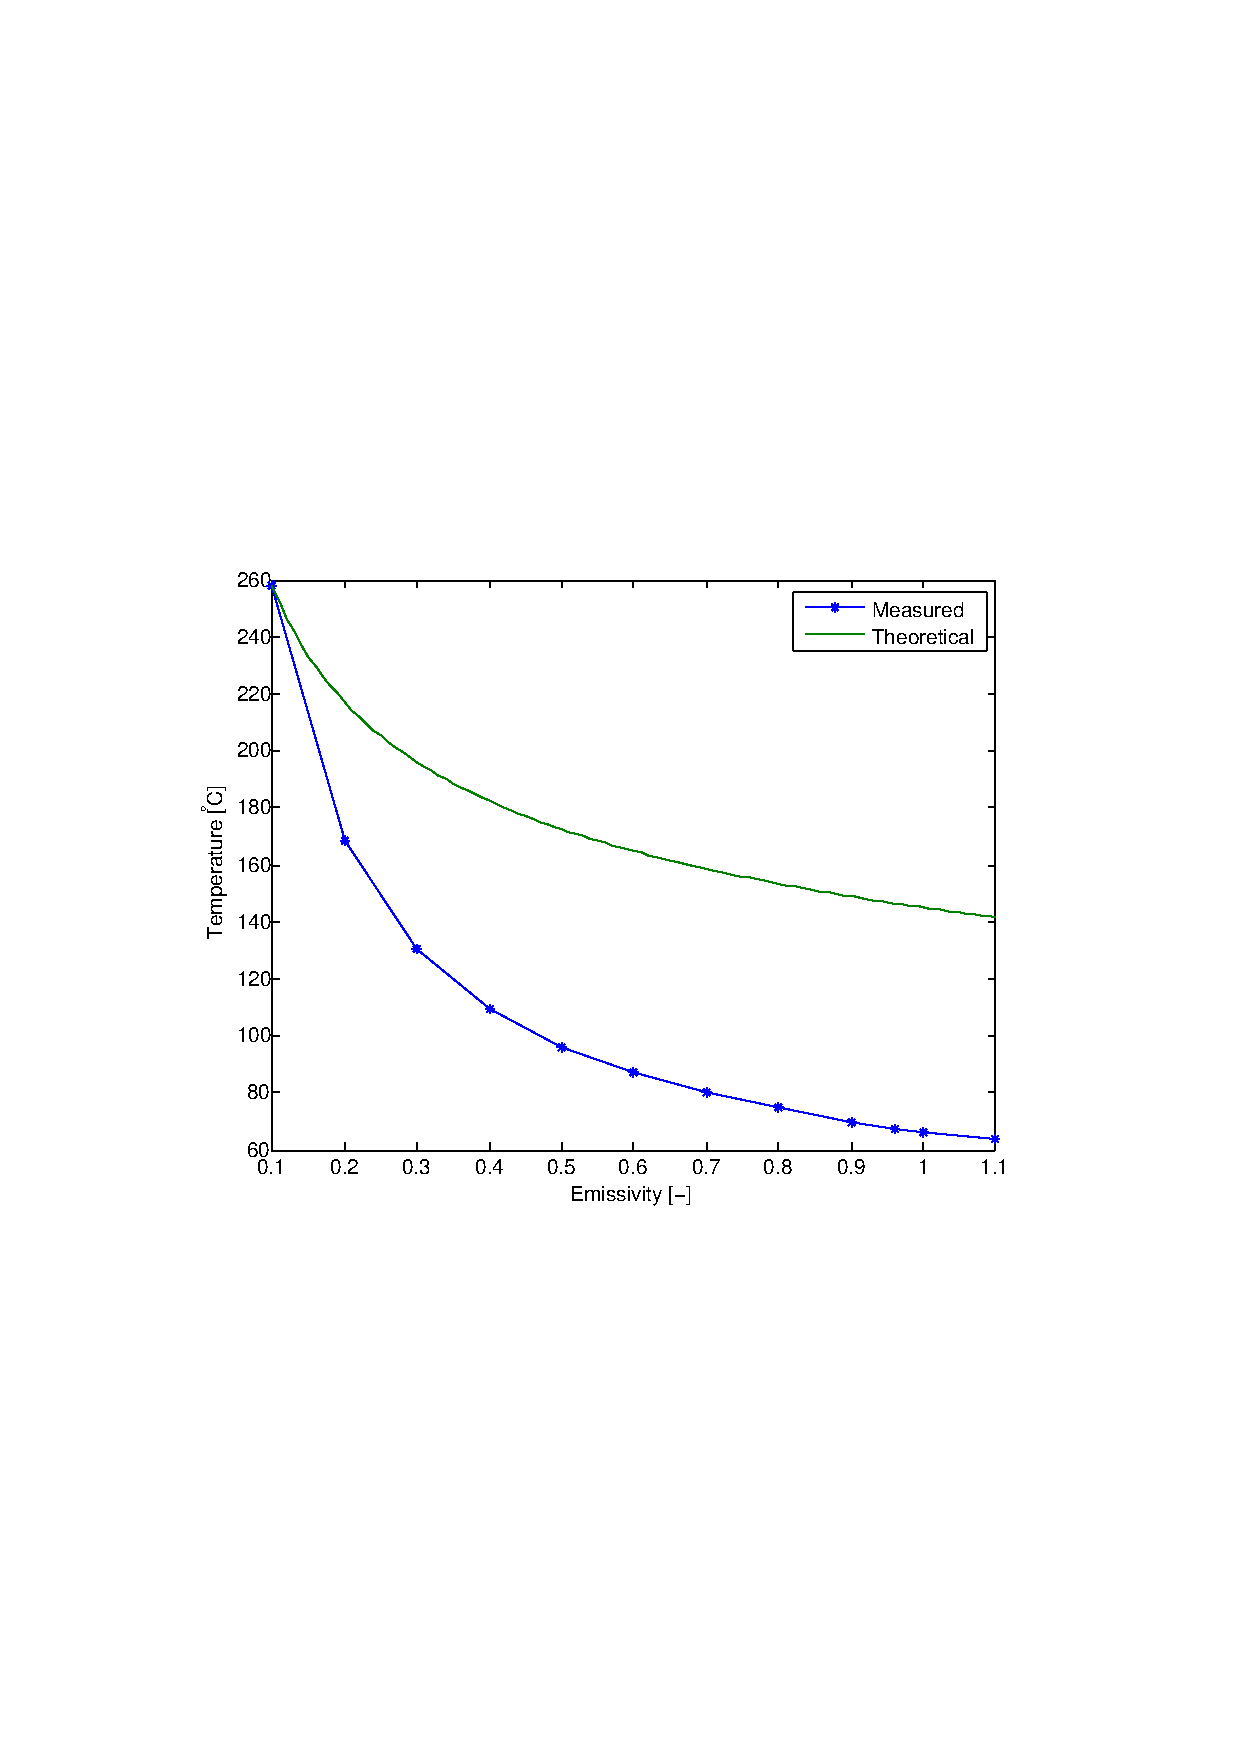
\includegraphics[trim=5cm 9cm 5cm 9cm,width=10cm]{../res/img/T_f(E).pdf} 
			\end{center}
			\caption{Zależność temperatury badanego obiektu od jego współczynnika
			emisyjności}
			\label{rys:pirE_T}
		\end{figure}
		
		Na rysunku \ref{rys:pirE_T} zamieszczone zostały wyniki uzyskanych pomiarów,
		oraz teoretyczny zgodny z równaniem \eqref{equ:temp} przebieg badanej
		zależności (stała $C$ wyznaczona na podstawie pierwszego punktu pomiarowego).
		Jak widać producent użył innej niż przytoczonej w sprawozdaniu zależności, co
		może wynikać np. z charakterystyki samej głowicy pomiarowej.
		
		Jako że wynik pomiaru temperatury silnie zależy od wartości współczynnika
		emisyjności badanego obiektu, oczywistym jest iż w celu wykonania dokładnego
		pomiaru potrzebna jest jego znajomość.
	\end{subsection}
	
	\newpage
	
	\begin{subsection}{Wpływ przesłon ograniczających bezpośrednie oddziaływanie
					promieniowania temperaturowego na pirometr}
		W celu wyznaczenia wpływu przeszkód wykonanych z różnych materiałów na
		dokładność pomiaru temperatury, pirometr został skierowany na obiekt o znanej
		emisyjności, którego temperatura została odnotowana. Następnie pomiary
		temperatury zostały powtórzone dla przeszkód na drodze między pirometrem a
		obiektem badanym. Jako przeszkody zostały użyte płytki ze szkła i pleksiglasu.
					
		Ponieważ pomiar pirometrem odbywa się na zasadzie pomiaru promieniowania
		emitowanego przez obiekt wszelkie przeszkody stojące na drodze optycznej
		między piromertem a badanym obiektem mogą zakłócać pomiar temperatury. Dzieje
		się tak dla tego że pewne materiały pochłaniają lub odbijają fale o długości z
		określonego zakresu. Tak stało się dla badanych materiałów, ponieważ odczyty
		pirometru, podczas gdy badany obiekt zasłaniała przeszkoda nie zdawały się
		różnić od odczytów temperatury tła.
		
		Wykonane pomiary dały wyniki:
		\begin{itemize}
		  \item Taśma bezpośrednio $65[^{\circ}C]$
		  \item Taśma przez szkło $25.5[^{\circ}C]$
		  \item Taśma przez pleksiglas $24.9[^{\circ}C]$
		\end{itemize}
		
	\end{subsection}
	
	\newpage
	
	\begin{subsection}{Rejestracja mierzonej temperatury i wyznaczenie odpowiedzi
					dynamicznej pirometru}
		W celu pomiaru reakcji czujnika na skoki wartości mierzonej temperatury, w
		oprogramowaniu DasyLab(karta pomiarowa) oraz Pyrometer(RS232) zostały
		połączone i ustawione odpowiednie konfiguracje do akwizycji danych z czujnika
		pomiarowego w czasie rzeczywistym. W obydwu przypadkach zebrane dane zostały
		przekierowane do plików celem późniejszego wykorzystania do wyznaczenia
		stałych czasowych czujnika.
		%Samą metodyką pomiaru parametrów dynamicznych
		%czujnika było zadawanie skoków temperatury mierzonej poprzez nagłe
		%zasłanianie drogi między obiektem którego temperatura była mierzona innym
		%obiektem o różnej temperaturze.
		Dane potrzebne do wyznaczenia parametów dynamicznych czujnika, to skoki
		wartości mierzonej przez pirometr temperatury.
		Skoki temperatury mierzonej zostały osiągnięte poprzez nagłe przesłanianie
		pola pomiarowego czujnika obiektami które charakteryzowały się różniącymi się
		współczynnikami emisyjności.
		\begin{figure}[!htb]
			\begin{center} 
				\includegraphics[trim=5cm 8cm 5cm 8cm,width=10cm]{../res/img/T_f(t).pdf} 
			\end{center}
			\caption{Przebiegi czasowe temperatury odczytywanej z czujnika podczas
			przesłaniania pola pomiarowego czujnika obiektami o różnej emisyjności}
			\label{rys:pirt_T}
		\end{figure}
		
		Z tak pobranych danych pomiarowych metodą graficzną zostały wyznaczone stałe
		czasowe czujnika:
		\begin{itemize}
		  \item Nagrzewania $\tau_n = 0.14[s]$
		  \item Ochładzania $\tau_o = 0.12[s]$
		\end{itemize}
	
	\end{subsection}
	
	\newpage
	
	\begin{subsection}{Nastawianie oraz odczyt parametrów pirometru z
					wykorzystaniem interfejsu portu szeregowego}
	Badany pirometr został wyposarzony w standardowy asynchroniczny interfejs
	szeregowy służący do modyfikowania parametrów pomiaru oraz odczytywania ich
	wartości. Parametry ramki danych:
	
	\begin{itemize}
	  \item Prędkość transmisji (baudrate) - 9600 bodów
	  \item 8 bitów danych
	  \item 1 bit stopu
	  \item brak kontroli parzystości
	  \item brak kontroli przepływu danych
	\end{itemize}
	
	Jedna z aplikacji używanych podczas laboratorium (Pyrometr) do
	odczytu danych z przetwornika pomiarowego korzystała z jego interfejsu
	szeregowego. Wszystkie komendy mające na celu uzyskanie od przetwornika pewnych
	informacji zaczynają się od pojedynczego znaku zapytania. Przykładowe komendy
	użyte podczas laboratorium:
	
	\begin{itemize}
	  \item ?T - zapytanie o aktualnie mierzoną temperaturę
	  \item ?E - zapytanie o aktualnie ustawioną wartość emisyjności obiektu
	  przyjmowanej do przeliczania odczytów głowicy na temperaturę
	  \item ?XU - zapytanie o identyfikator urządzenia
	\end{itemize}
	
	Warto nadmienić, iż ważnym jest aby każda komenda kończyła się znakami nowej
	linii oraz powrotu karetki, ponieważ w przypadku ich braku przetwornik nie był
	w stanie poprawnie interpretować komend, w związku z czym na żadną nie
	odpowiadał.
	
	\end{subsection}
	
\end{section}

\newpage

\begin{section}{Wnioski}
	Dokładność pomiarów wykonanych pirometrem jest silnie zależna od wielu
	czynników, jak odległość czujnika od mierzonego obiektu, znajomość materiału z
	którego wykonany jest obiekt (współczynnik emisyjności), temperatura tła i
	wiele innych. W związku z tym zastosowanie pirometrów do pomiaru temperatury
	jest bardzo uciążliwe a zatem ograniczone do wąskiej klasy zastosowań, które
	wymagają np. braku kontaktu czujnika z mierzonym obiektem, czy bardzo wysokie
	temperatury badanych obiektów.
\end{section} 

\begin{section}{Wykaz aparatury}   
	\begin{enumerate}
	  \item Komputer z systemem operacyjnym Windows XP lub wyższym i portem COM
	  \item Karta pomiarowa NI6221 wraz z płytką łączeniową
	  \item Oprogramowanie DASY Lab wraz ze sterownikami do karty (NI - DAQmx)
	  \item Oprogramowanie do obsługi interfejsu portu szeregowego,
	  \item Pirometr MID02 wraz z układem zasilania połączony kablem RS232C z
	  komputerem
	  \item Obiekty pomiaru temperatury
	  \item Kalibrator temperatury wraz z czujnikami: termorezystorem Pt100 i
	  termoparą.
	\end{enumerate}
\end{section}

\end{document}